\section{HITS}

کدهای ابتدایی این قسمت بسیار شبیه به حالت‌های قبلی هستند. در این الگوریتم، 
دوربین‌ها به عنوان
hub
 و زمان‌ها به عنوان 
auhtority
در نظر گرفته‌شده‌اند. سپس با استفاده از تجزیه‌ی 
SVD
الگوریتم 
HITS
را پیاده‌سازی کردم. نتایج نهایی به صورت زیر بودند: 

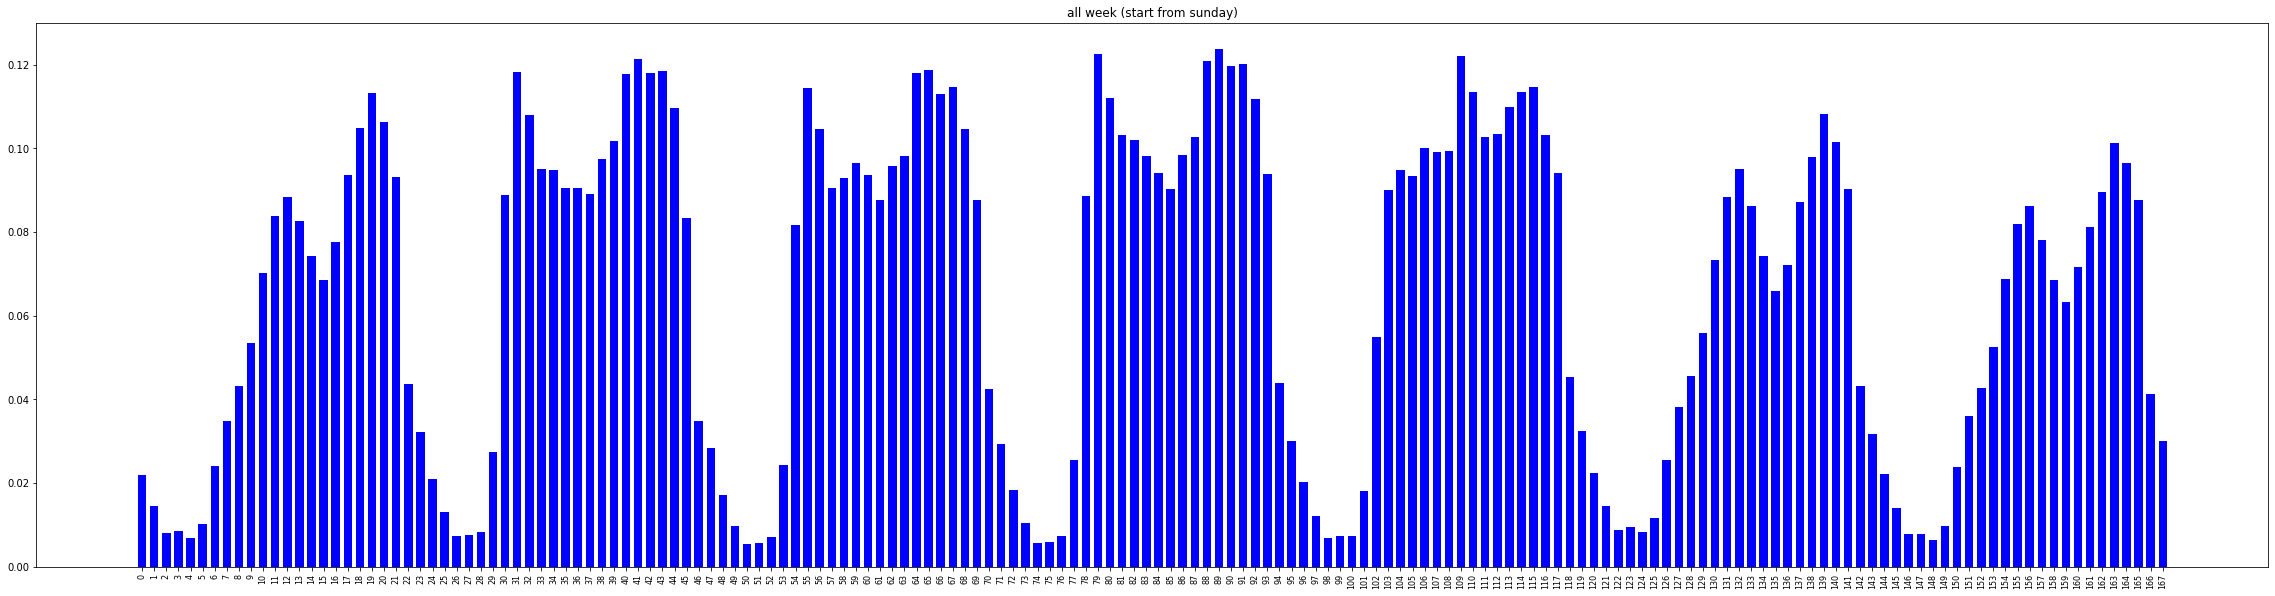
\includegraphics[scale=0.2]{images/HITS/1.png}

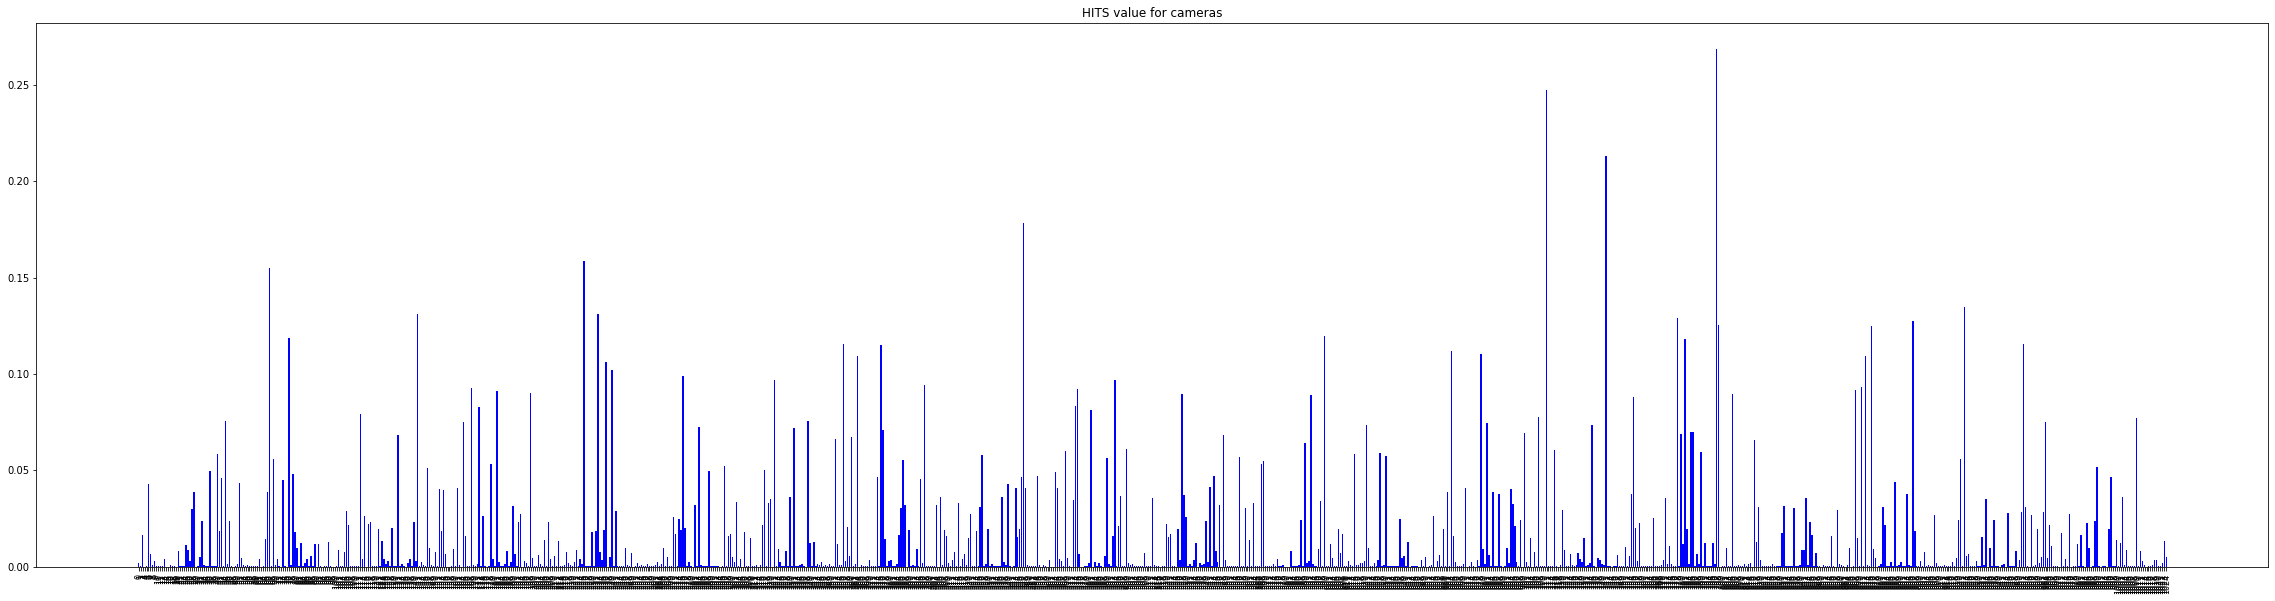
\includegraphics[scale=0.2]{images/HITS/2.png}


\subsection{تحلیل نتایج}
مقادیر این دو نمودار، به ما زمان‌ها یا دوربین‌هایی را نشان‌ می‌دهند که به احتمال بیشتری ثبت می‌کنند. در واقع این نمودار دوربین‌ها می‌تواند 
به ما بگوید که کدام دوربین‌ها در ساعات پرتردد احتمال ثبت بیشتری دارند. اما این اطلاعات خیلی سود‌آور نیست. 
اما در مورد زمان‌ها، نمودار‌ها اطلاعاتی دارند که با شهود ما سازگار است. همانطوری که می‌بینید، روز‌های دوشنبه تا 
چهارشنبه حالت 
U
شکل دارند، که این یعنی دو پیک ترافیکی یکی در صبح و یکی در شب داریم. اما این 
الگو در روز پنج شنبه، احتمالا به دلیل تعطیلی مدارس از بین می‌رود. سپس 
در روز‌های جمعه و شنبه و یک‌شنبه، همانطوری که می‌بینید پیک شب قوی تر بوده است، که دلیل آن 
تعطیلی این سه روز است، که مردم بیشتر در شب تردد دارند (تعطیلی مدارس و ادارات). 
